% Lights Out: a press toggles a plus shape; a quiet pattern of the 5x5 board.
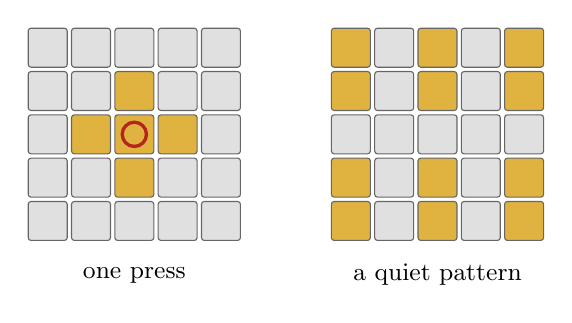
\begin{tikzpicture}[scale=0.55]
\filldraw[fill=black!12,draw=black!60,rounded corners=1pt] (0,0) rectangle ++(0.9,0.9);
\filldraw[fill=black!12,draw=black!60,rounded corners=1pt] (1,0) rectangle ++(0.9,0.9);
\filldraw[fill=black!12,draw=black!60,rounded corners=1pt] (2,0) rectangle ++(0.9,0.9);
\filldraw[fill=black!12,draw=black!60,rounded corners=1pt] (3,0) rectangle ++(0.9,0.9);
\filldraw[fill=black!12,draw=black!60,rounded corners=1pt] (4,0) rectangle ++(0.9,0.9);
\filldraw[fill=black!12,draw=black!60,rounded corners=1pt] (0,-1) rectangle ++(0.9,0.9);
\filldraw[fill=black!12,draw=black!60,rounded corners=1pt] (1,-1) rectangle ++(0.9,0.9);
\filldraw[fill=Goldenrod!85,draw=black!60,rounded corners=1pt] (2,-1) rectangle ++(0.9,0.9);
\filldraw[fill=black!12,draw=black!60,rounded corners=1pt] (3,-1) rectangle ++(0.9,0.9);
\filldraw[fill=black!12,draw=black!60,rounded corners=1pt] (4,-1) rectangle ++(0.9,0.9);
\filldraw[fill=black!12,draw=black!60,rounded corners=1pt] (0,-2) rectangle ++(0.9,0.9);
\filldraw[fill=Goldenrod!85,draw=black!60,rounded corners=1pt] (1,-2) rectangle ++(0.9,0.9);
\filldraw[fill=Goldenrod!85,draw=black!60,rounded corners=1pt] (2,-2) rectangle ++(0.9,0.9);
\filldraw[fill=Goldenrod!85,draw=black!60,rounded corners=1pt] (3,-2) rectangle ++(0.9,0.9);
\filldraw[fill=black!12,draw=black!60,rounded corners=1pt] (4,-2) rectangle ++(0.9,0.9);
\filldraw[fill=black!12,draw=black!60,rounded corners=1pt] (0,-3) rectangle ++(0.9,0.9);
\filldraw[fill=black!12,draw=black!60,rounded corners=1pt] (1,-3) rectangle ++(0.9,0.9);
\filldraw[fill=Goldenrod!85,draw=black!60,rounded corners=1pt] (2,-3) rectangle ++(0.9,0.9);
\filldraw[fill=black!12,draw=black!60,rounded corners=1pt] (3,-3) rectangle ++(0.9,0.9);
\filldraw[fill=black!12,draw=black!60,rounded corners=1pt] (4,-3) rectangle ++(0.9,0.9);
\filldraw[fill=black!12,draw=black!60,rounded corners=1pt] (0,-4) rectangle ++(0.9,0.9);
\filldraw[fill=black!12,draw=black!60,rounded corners=1pt] (1,-4) rectangle ++(0.9,0.9);
\filldraw[fill=black!12,draw=black!60,rounded corners=1pt] (2,-4) rectangle ++(0.9,0.9);
\filldraw[fill=black!12,draw=black!60,rounded corners=1pt] (3,-4) rectangle ++(0.9,0.9);
\filldraw[fill=black!12,draw=black!60,rounded corners=1pt] (4,-4) rectangle ++(0.9,0.9);
\draw[very thick,BrickRed] (2.45,-1.55) circle (0.28);
\filldraw[fill=Goldenrod!85,draw=black!60,rounded corners=1pt] (7,0) rectangle ++(0.9,0.9);
\filldraw[fill=black!12,draw=black!60,rounded corners=1pt] (8,0) rectangle ++(0.9,0.9);
\filldraw[fill=Goldenrod!85,draw=black!60,rounded corners=1pt] (9,0) rectangle ++(0.9,0.9);
\filldraw[fill=black!12,draw=black!60,rounded corners=1pt] (10,0) rectangle ++(0.9,0.9);
\filldraw[fill=Goldenrod!85,draw=black!60,rounded corners=1pt] (11,0) rectangle ++(0.9,0.9);
\filldraw[fill=Goldenrod!85,draw=black!60,rounded corners=1pt] (7,-1) rectangle ++(0.9,0.9);
\filldraw[fill=black!12,draw=black!60,rounded corners=1pt] (8,-1) rectangle ++(0.9,0.9);
\filldraw[fill=Goldenrod!85,draw=black!60,rounded corners=1pt] (9,-1) rectangle ++(0.9,0.9);
\filldraw[fill=black!12,draw=black!60,rounded corners=1pt] (10,-1) rectangle ++(0.9,0.9);
\filldraw[fill=Goldenrod!85,draw=black!60,rounded corners=1pt] (11,-1) rectangle ++(0.9,0.9);
\filldraw[fill=black!12,draw=black!60,rounded corners=1pt] (7,-2) rectangle ++(0.9,0.9);
\filldraw[fill=black!12,draw=black!60,rounded corners=1pt] (8,-2) rectangle ++(0.9,0.9);
\filldraw[fill=black!12,draw=black!60,rounded corners=1pt] (9,-2) rectangle ++(0.9,0.9);
\filldraw[fill=black!12,draw=black!60,rounded corners=1pt] (10,-2) rectangle ++(0.9,0.9);
\filldraw[fill=black!12,draw=black!60,rounded corners=1pt] (11,-2) rectangle ++(0.9,0.9);
\filldraw[fill=Goldenrod!85,draw=black!60,rounded corners=1pt] (7,-3) rectangle ++(0.9,0.9);
\filldraw[fill=black!12,draw=black!60,rounded corners=1pt] (8,-3) rectangle ++(0.9,0.9);
\filldraw[fill=Goldenrod!85,draw=black!60,rounded corners=1pt] (9,-3) rectangle ++(0.9,0.9);
\filldraw[fill=black!12,draw=black!60,rounded corners=1pt] (10,-3) rectangle ++(0.9,0.9);
\filldraw[fill=Goldenrod!85,draw=black!60,rounded corners=1pt] (11,-3) rectangle ++(0.9,0.9);
\filldraw[fill=Goldenrod!85,draw=black!60,rounded corners=1pt] (7,-4) rectangle ++(0.9,0.9);
\filldraw[fill=black!12,draw=black!60,rounded corners=1pt] (8,-4) rectangle ++(0.9,0.9);
\filldraw[fill=Goldenrod!85,draw=black!60,rounded corners=1pt] (9,-4) rectangle ++(0.9,0.9);
\filldraw[fill=black!12,draw=black!60,rounded corners=1pt] (10,-4) rectangle ++(0.9,0.9);
\filldraw[fill=Goldenrod!85,draw=black!60,rounded corners=1pt] (11,-4) rectangle ++(0.9,0.9);
\node[font=\small] at (2.45,-4.8) {one press};
\node[font=\small] at (9.45,-4.8) {a quiet pattern};
\end{tikzpicture}
